\documentclass{HW}

\newcommand{\hwtitle}{آزمایش سه}
\newcommand{\studentname}{رادین شایانفر}
\newcommand{\studentnumber}{9731032}

\usepackage[top=30mm, bottom=30mm, left=25mm, right=25mm]{geometry}
\usepackage{amsthm,amssymb,amsmath,amsfonts}
\usepackage{fancyhdr}
\usepackage{changepage}
\usepackage{enumitem}
\usepackage{listings}
\usepackage[table]{xcolor}
\usepackage{fontspec}

\newfontfamily{\ttconsolas}{Consolas}

\definecolor{codegreen}{rgb}{0,0.6,0}
\definecolor{codegray}{rgb}{0.5,0.5,0.5}
\definecolor{codepurple}{rgb}{0.58,0,0.82}
\definecolor{backcolour}{rgb}{0.95,0.95,0.92}

\lstset{
  backgroundcolor=\color{backcolour},   
  commentstyle=\color{codegreen},
  keywordstyle=\color{magenta},
  numberstyle=\tiny\color{codegray},
  stringstyle=\color{codepurple},
  basicstyle=\ttconsolas\footnotesize,
  breakatwhitespace=false,         
  breaklines=true,                 
  captionpos=b,                    
  keepspaces=true,  
  numbers=left,                    
  numbersep=5pt,                  
  showspaces=false,                
  showstringspaces=false,
  showtabs=false,                  
  tabsize=4
}

\usepackage{array,multirow}

\usepackage{tikz}
\usetikzlibrary{trees}

% بسته‌‌ای برای ظاهر شدن شکل‌ها و تصاویر متن
\usepackage{graphicx}
\usepackage{color}
%بسته‌ای برای تنظیم فاصله عمودی خط‌های متن
\usepackage{setspace}

\usepackage[pagebackref=false,colorlinks,urlcolor=cyan,linkcolor=blue,citecolor=red]{hyperref}

\hypersetup{
    pdftitle={\hwtitle - \studentname - شماره دانشجویی: \studentnumber},
    bookmarks=true,
    pdfauthor={Radin Shayanfar},
}

% بسته‌ لازم برای تنظیم سربرگ‌ها
\usepackage{fancyhdr}

\usepackage{ptext} 
\usepackage{xepersian}

\doublespacing

\SepMark{-}
\settextfont[Scale=1.2]{B Nazanin}
\setlatintextfont{Times New Roman}
\renewcommand{\labelitemi}{$\bullet$}

\newcounter{mynumber}
\setcounter{mynumber}{1}
\newcommand{\mynum}{\arabic{mynumber}\stepcounter{mynumber}}

\newenvironment{question}{%
\medskip%
\par%
\noindent%
\textbf{سوال \mynum- \space}%
\smallskip
%\par\noindent\ignorespaces
\begin{adjustwidth}{7mm}{}
}{%
\end{adjustwidth}
\par\medskip
}

\fancypagestyle{first_page}{
\fancyhf{}
\fancyhead[C]{\raisebox{3ex}{\large \bfseries \hwtitle}}
\fancyhead[LO,LE]{\textbf{\studentname} \\
شماره دانشجویی: \studentnumber
\vspace{0.2mm}}
\fancyfoot[C]{\thepage{}}
\renewcommand{\headrulewidth}{1.2pt}
}

\fancypagestyle{pages}{
\fancyhf{}
\fancyhead[R]{\leftmark}
\fancyfoot[C]{\thepage{}}
\renewcommand{\headrulewidth}{1.2pt}
}

\begin{document}
\pagestyle{pages}
\thispagestyle{first_page}

\section{آنالیز کد سریال}

ابتدا \lr{Hotspot}های برنامه را بررسی می‌کنیم تا متوجه شویم چه قسمت‌هایی از برنامه بیشترین زمان اجرا را به خود اختصاص داده‌اند.

برای این کار با تبدیل مقدار \lr{VERYBIG} به ۱۰ هزار و تعداد تکرارهای برنامه به ۱، آن را به کمک \lr{VTune} آنالیز می‌کنیم. پس از آنالیز شدن برنامه، با دو بار کلیک بر روی تابع \lr{main}، به سورس کد برنامه (شکل \ref{fig:hotspots}) می‌رویم و خطوطی که بیشترین زمان اجرا را به خود اختصاص داده‌اند را می‌بینیم.


\begin{figure}[ht!]
\begin{center}
	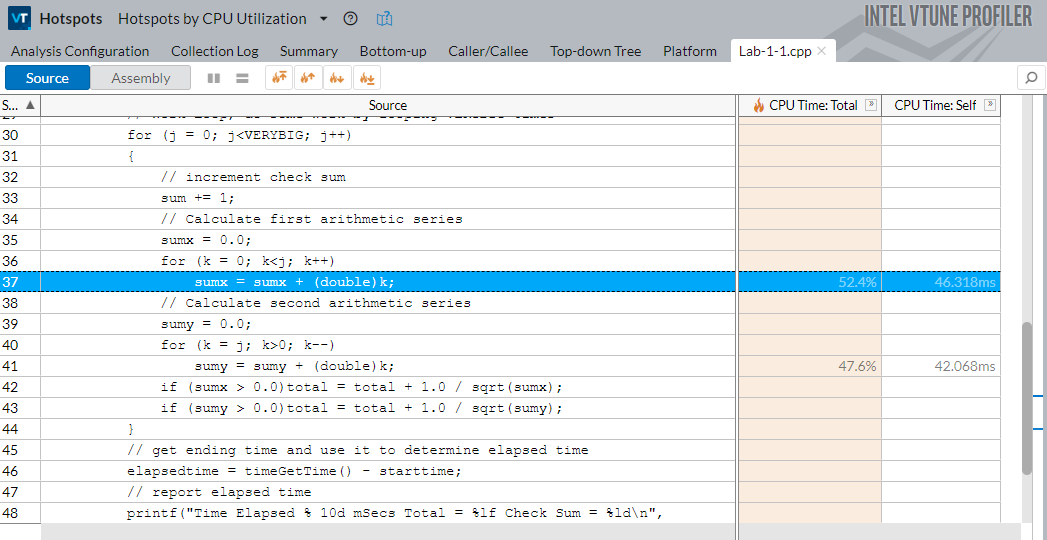
\includegraphics[width=15cm]{images/hotspots}
\end{center}
\caption{نتایج آنالیز با \lr{VTune}}
\label{fig:hotspots}
\end{figure}

\section{موازی‌سازی به کمک \lr{OpenMP}}

پس از مشاهده قسمت‌هایی از برنامه که زمان اجرای آن‌ها طولانی‌تر است، سعی می‌کنیم با موازی‌سازی این بخش‌ها تسریع بگیریم. با گذاشتن خط زیر پیش از حلقه \lr{work}، اجراهای آن را موازی می‌کنیم.

\begin{latin}
%\begin{minipage}{\linewidth}
\begin{lstlisting}[language=C]
#pragma omp parallel for
\end{lstlisting}
%\end{minipage}
\end{latin}

مشاهده می‌شود که در این حالت زمان اجرای برنامه حتی بیشتر شده است و برنامه به درستی اجرا نمی‌شود (مقدار متغیرهای \lr{sum} و \lr{total} درست نیست).

\section{دیباگ و رفع خطاها}

با ابزار \lr{Inspector} و کاهش دادن مقدار \lr{VERYBIG} به هزار، برنامه را تحلیل می‌کنیم.

همانطور که در شکل
\ref{fig:datarace}
می‌بینیم، برنامه دارای شرایط مسابقه برای متغیرهای مشترک (\lr{sum}، \lr{total}، \lr{sumx}، \lr{sumy} و \lr{k}) است.

\begin{figure}[ht!]
\begin{center}
	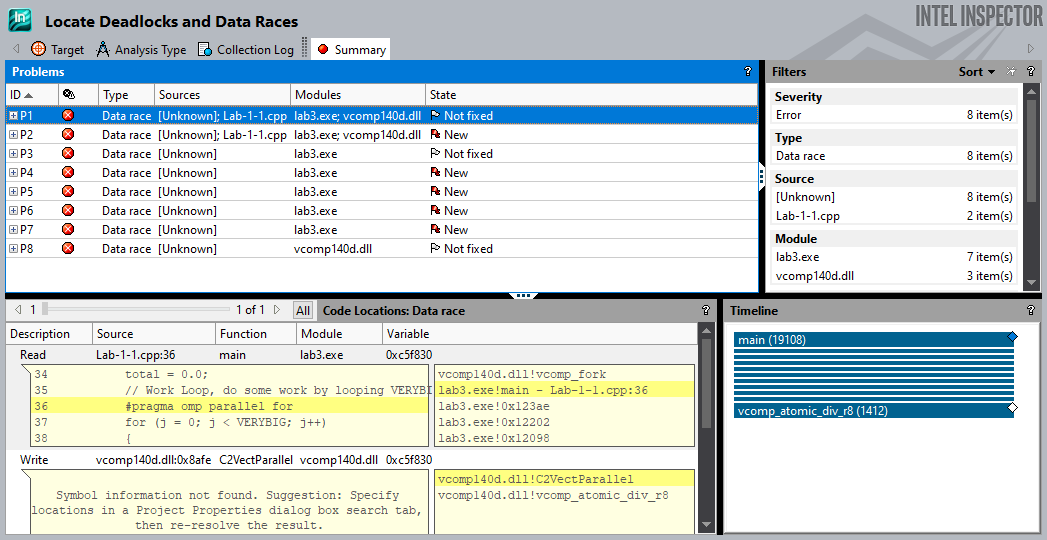
\includegraphics[width=15cm]{images/datarace}
\end{center}
\caption{وجود شرایط مسابقه برای متغیرهای مشترک بین نخ‌ها}
\label{fig:datarace}
\end{figure}

با استفاده از خط زیر، متغیرهایی که می‌توانند خصوصی باشند را خصوصی می‌کنیم. همچنین متغیرهایی که باید مقدار آن‌ها بین همه نخ‌ها مشترک باشد را می‌توانیم با استفاده از عبارت \lr{reduction}، جلوی شرایط مسابقه آن را بگیریم.

\begin{latin}
%\begin{minipage}{\linewidth}
\begin{lstlisting}[language=C]
#pragma omp parallel for private(sumx, sumy, k) reduction(+:sum, total)
\end{lstlisting}
%\end{minipage}
\end{latin}


\section{تنظیم و سرعت‌بخشیدن به برنامه \lr{OpenMP}}

با آنالیز برنامه به کمک \lr{VTune} مطابق شکل
\ref{fig:tune-bad}،
مشاهده می‌کنیم که کار به صورت نامتوازن بین نخ‌ها پخش شده است. در واقع برخی نخ‌ها زودتر کارشان به اتمام می‌رسد و به ناچار منتظر دیگر نخ‌ها می‌مانند. همچنین در شکل
\ref{fig:tune-bad2}
می‌بینیم که مدت زمان بسیار کمی هر ۸ نخ همزمان با هم فعال هستند (ستون سمت راست) و این به معنی استفاده نامناسب از تمام توان پردازشی پردازنده است.

\begin{figure}[ht!]
\begin{center}
	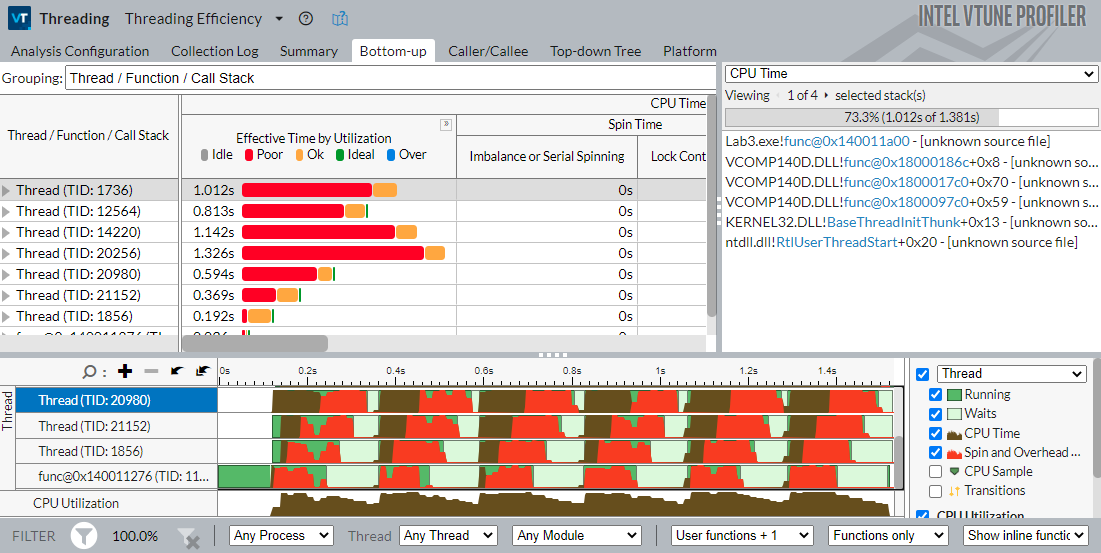
\includegraphics[width=15cm]{images/tune-bad}
\end{center}
\caption{پخش نامتوازن کار بین نخ‌ها}
\label{fig:tune-bad}
\end{figure}

\begin{figure}[ht!]
\begin{center}
	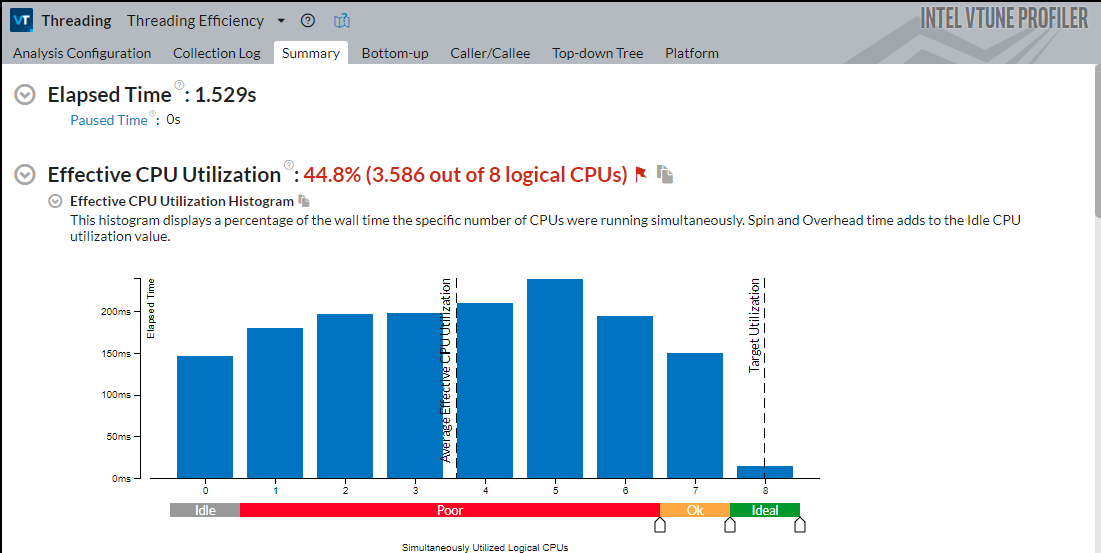
\includegraphics[width=15cm]{images/tune-bad2}
\end{center}
\caption{عدم استفاده از تمام توان پردازشی پردازنده به علت پخش نامتوازن کارها}
\label{fig:tune-bad2}
\end{figure}

این پخش نامتوازن به علت محاسبات بیشتر نخ‌های پایانی در حلقه \lr{k} است. با استفاده از عبارت زیر می‌توانیم پخش کارها را متوازن کنیم.

\begin{latin}
%\begin{minipage}{\linewidth}
\begin{lstlisting}[language=C]
#pragma omp parallel for private(sumx, sumy, k) \
reduction(+:sum, total) schedule(dynamic, 2000)
\end{lstlisting}
%\end{minipage}
\end{latin}

با آنالیز مجدد کارکرد نخ‌ها با استفاده از \lr{VTune}، می‌بینیم که پخش کارها بسیار متوازن‌تر است و به بهره‌وری ایده‌آل بسیار نزدیک‌تر شده‌ایم (شکل‌های
\ref{fig:tune-good}
و
\ref{fig:tune-good2})

\begin{figure}[ht!]
\begin{center}
	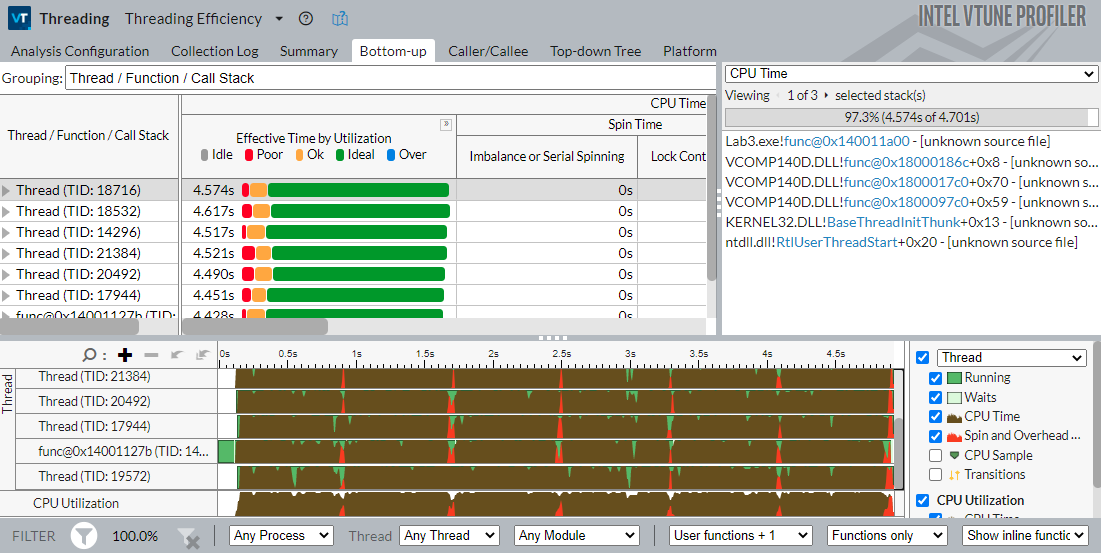
\includegraphics[width=15cm]{images/tune-good}
\end{center}
\caption{پخش بسیار بهتر کارها پس از استفاده از \lr{schedule(static)} و با \lr{chunk size} برابر ۲۰۰۰}
\label{fig:tune-good}
\end{figure}

\begin{figure}[ht!]
\begin{center}
	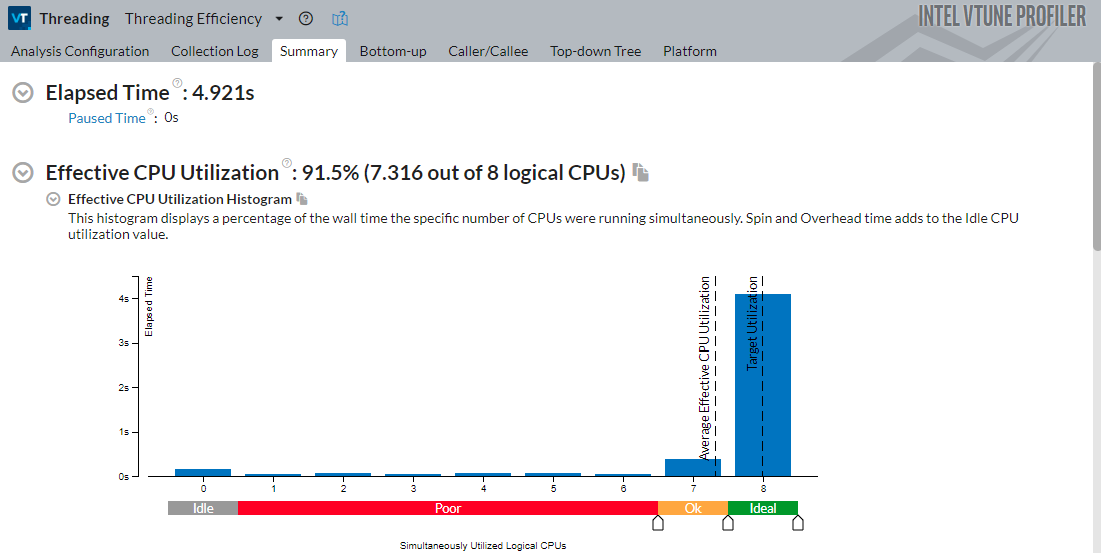
\includegraphics[width=15cm]{images/tune-good2}
\end{center}
\caption{نزدیک شدن به میزان بهره‌وری ایده‌آل پردازنده}
\label{fig:tune-good2}
\end{figure}

\end{document}
